\documentclass[a4paper,12pt]{article}
\usepackage{mathtools, amsmath, listings,graphicx}
\graphicspath{ {images/} }
\begin{document}
\lstset{language=Python}

\title{Paths: a Powerful Graph Invariant with Interesting Limitations - First Semester Report}
\author{Grady Ward}

\maketitle

In searching for a polynomial time-complexity solution to the graph isomorphism problem, many researchers have focused on, \emph{vertex invariants}, numerical properties calculated over a vertex of a graph that can be deterministically calculated, regardless of how the graph is represented or labeled. This article will aim to describe the descriptive power and information density of the \(Paths(p, v)\) function, a vertex invariant that counts the number of closed paths of length \(p\) through a vertex \(v\). The \(Paths\) function, in order to be applied to the graph isomorphism problem, is used to construct an algebraic graph invariant, with the application of sorting to the results of individual vertex \(Paths\) results.

Though research into the descriptive power of this function has shown that it does not fully determine the graph, the lines of inquiry have proven to be fruitful in describing patterns of graph behavior that a casual observer would not anticipate.  Additionally, the invariant's descriptive power can be computationally described in a way that is meaningful, and shows that for its time complexity, it is an incredibly discriminatory algorithm.  Finally, this article will hope to address the various lines of inquiry that will hopefully be addressed in further research on this topic, including a systematic analysis of the classes of graphs that the Paths function is effective for, and those for which it is insufficient to prove isomorphism.

\section{Background}

To begin a discussion of this work, we must first establish a mutual understanding of the functions that we are discussing, the scope of existing research on this topic, and an appropriate category of graphs to examine.

\subsection{Definitions}

In this analysis, we will be examining \(undirected\) graphs that do not contain multi-edges nor loops.  Any graph under these three constraints can be represented as a symmetric adjacency matrix, with zeros along the diagonal, and ones or zeroes in the remaining locations denoting an edge or disjoint vertices respectively. We will regularly reference this matrix as \(A\) with no additional annotation.

The vertex invariant we are going to examine (\(Paths(p, v)\)) is the number of closed paths of a length \(p\) that contain the vertex \(v\). A path is a sequence of vertices such that each vertex shares an edge with the next one. A Path can be notated by the sequence of the vertices that are visited (e.g. ABCDE or BACAB). A Path is \emph{closed} if the first and last vertex in their traversal sequence are the same. Note that though \(ABCDE\) and \(EDCBA\) describe the same edges, they are distinct paths: even though an undirected graph doesn't have directional edges, paths maintain the order of the edges they traverse.

For this article, when we describe a path as a geometric polygon (such as a triangle, quadrilateral, pentagon, etc.), we will define to be a closed path such that the vertices of the path are non-repeating (aside from the first and last, as we assume that it is closed). Thus, \(ABABA\) does not form a quadrilateral, even though it is a closed path of length four. Note that this path could equally well be described as \(BABAB\), as closed paths are inherently cyclic, and do not demand a starting vertex.  Additionally, we will assume that unlike a path, a polygon's directionality does not matter (thus the polygon ABCA is the same as the polygon ACBA). 

\subsection{Computation of the Paths Function}

The \(Paths(p, v)\) function counts the number of unique closed paths that pass through a given vertex, \(v\).  This information can be easily computed using \(A\). Just as the entries of \(A^1\) represent the existence of paths of length 1 between two vertices (edges), the entries of \(A^p\) represent the number of paths of length \(p\) between any two vertices (by examining the row and column corresponding to two vertices). Thus, to find the number of closed paths of length \(p\) that contain a given vertex \(v\), we simply need to calculate: \[Paths(p, v) = A^p[v, v]\]Where \(v\) is being used interchangeably here with its represented position within the adjacency matrix. Thus, calculating a specific value of \(Paths(p, v)\) can occur in the time it takes to exponentiate \(A\) to the power \(p\).  Though it is a well known result that matrix multiplication can be done in faster than \(O(n^3)\) time, we will be using the na�ve assumption that matrix multiplication runs in \(O(n^3)\) in order to make the computational complexity calculations more accessible.  Under that assumption, it is clear that calculating \(Paths(p, v)\) will occur in \(O(pv^3)\) time. This is well within polynomial time, so long as we request a polynomial number of values from \(Paths(p, v)\). Thus we can consider this invariant one in the traditional vein of looking for polynomial invariants with the broad aim of solving GI in polynomial time, though we have already established that it does not uniquely determine isomorphism.

\subsection{Expansion to a Paths Object}

Since \(Paths(p, v)\) is a function that operates over a vertex, we will be examining a slightly modified version of the function which operates over a graph: \(Paths(P, G)\).  \(Paths(P, G)\) produces a graph invariant that is related to its vertex invariant function by a simple translation.  \(Paths(p, v)\) is calculated for all \(v\in G, p \leq P\), resulting in \(v\) vectors, each of which has \(P\) elements, representing the paths function when calculated at that node for each successive value of \(p\). Since vectors are comparable objects, we can sort them, and return back a list of these vectors as a graph invariant, one that is computable and invariant to changes in vertex relabeling or adjacency matrix ordering. A skeptical reader should convince themselves that this holds true, even when two of the vectors to be sorted are identical, the resulting \(Paths\) object is valid and deterministically constructed from the graph.

%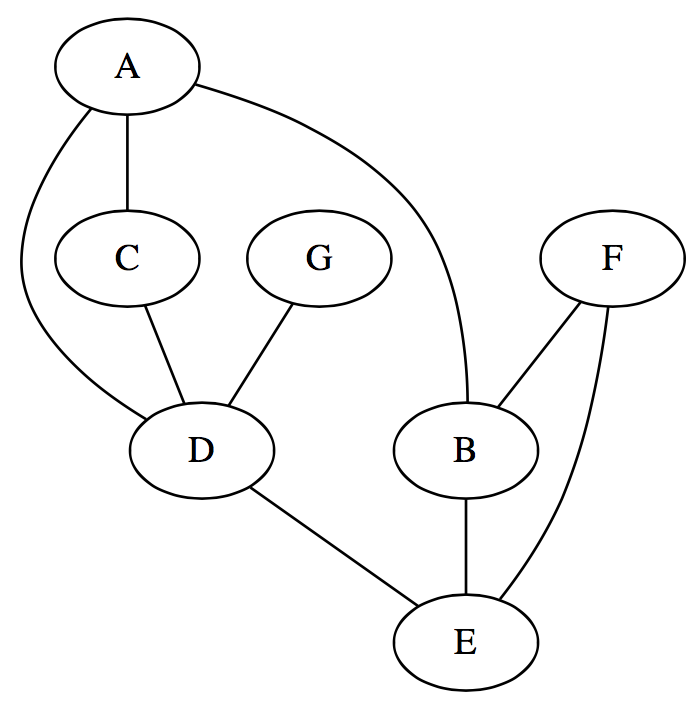
\includegraphics[scale=0.4]{examplegraph}
%\( A = \left ( \begin{array}{ccccccc}
%0 & 1 & 1 & 1 & 0 & 0 & 0 \\1 & 0 & 0 & 0 & 1 & 1 & 0 \\1 & 0 & 0 & 1 & 0 & 0 & 0 \\1 & 0 & 1 & 0 & 1 & 0 & 1 \\0 & 1 & 0 & 1 & 0 & 1 & 0 \\0 & 1 & 0 & 0 & 1 & 0 & 0 \\0 & 0 & 0 & 1 & 0 & 0 & 0\end{array} \right)\) 

\subsection{Co-Paths and Isomorphism}

Finally, two Graphs are said to be Co-Paths if they produce the same \(Paths\) object.  Since the Paths function is invariant to labeling and positioning, all isomorphic graphs are Co-Paths. However, a broader question is implied by this implication: does the reverse hold? Does Co-Paths determine isomorphism?  The answer turns out to be no, but the line of inquiry that leads to this result is worth examining, and leads us to a broader understanding and appreciation for the discriminatory power of the \(Paths\) function with respect to isomorphic graphs.

\section{Theoretical Work this Semester}
\subsection {Establishing Intuition: Paths and Polygon Functions}

The \(Paths(p, v)\) function has a very convenient geometric interpretation for small values of \(p\). This interpretation relies on the \(Polygon\) Function: \(Polygon(p, v) = \) \emph{Number of distinct Polygons of size p that contain v as a vertex}.

For small values of \(p\), we can express \(Polygon(p, v)\) in terms of \(Paths(p, v)\):

\begin{itemize}
    \item{Both invariants are uniform for all vertices for \(p = 0\) and \(p = 1\), as every vertex is trivially on a path to itself (so a path of size zero travels through it) and we have specified that there are no loops in the graph, thus there cannot be any edges that connect two of the same vertex.  Thus for all \(v\), \(Paths(0, v) = Polygon(0, v) = 1\) and \(Paths(1, v) =  Polygon(1, v) = 0\).}
    \item{For \(p = 2\), we know that \(Paths(2, v)\) is equivalent to the number of nodes that \(v\) shares an edge with. This number is called the degree of the node, and is often referred to as the "base invariant". We also know that this must equal \(Polygon(2, v)\), as a closed path of length two in a graph without loops must contain two distinct vertices.}
    \item{For \(p = 3\) we know that the only way to have a closed path of length three on the type of graph that we have described is to have three different edges (and three different vertices) form a triangle.  Thus, we know that \(p = 3\) is related to the number of triangles that a vertex is a part of.  However, since we are counting all possible combinatorial possibilities when we are describing our \(Paths(p, v)\) function, we need to take orientation into account.  That means that the path \(ABCA\) is fundamentally distinct from the counter directional path that visits the same nodes in the reverse order: \(ACBA\).  Though for \(p < 3, Paths(p, v) = Polygon(p, v)\), we know that for \(p = 3, \frac{Paths(3, v)}{2} = Polygon(3, v)\).}
     \item{The interpretation for \(p = 4\) is less intuitive, but some simple examination yields that it is the number of quadrilaterals that contain \(v\) when one subtracts off the possibility of repeating vertices.  Unlike \(p \leq 3\) and below, calculating \(Polygon(4, v)\) simply using values of \(Paths(x, v)\) is not possible unless you have the degrees of adjacent nodes to \(v\) (information not directly encoded into the paths function).  Using external information you could calculate the number of quadrilaterals that \(v\) is a part of.  Here we see the beginning of a divergence, of a differentiation between the polygon driven interpretation of \(Paths(p, v)\), and the more "combinatorial" reality.}
\end{itemize}

Examination beyond \(p = 4\) yields a similar picture: at each point in time, you need additional information (an increasing amount of it, too) in order to successfully calculate \(Polygons(p, v)\), even given unrestricted access to \(Paths(p, v\) for all p and v. A critical reader will have already come to the conclusion of this section, rooted in complexity theory.  If our graph is of size \(V\), we know that the calculation of \(Polygon(V, v)\) is the same for all \(v\) in the graph, as each vertex must be included exactly once on a closed path of length \(V\). This type of path is also called a \emph{Hamiltonian Cycle}, and its computation is known to be in NP-Complete.  If we hope that \(Paths\) offers easily computable access to lots of information about our graph, its divergence from \(Polygon(p, v)\) and \(Paths(p, v)\) is critical, as it thankfully does not imply that computing values of \(Paths\) is in the same complexity class as known intractable problems.

\subsection{Information of Paths and the Chromatic Polynomial}

One of the most discriminatory polynomial time algorithms for ruling out graph isomorphism is the Chromatic Polynomial of the graph's adjacency matrix A.  It is a well proven result that shuffling the order of the vertices in the representation of a given graph as an Adjacency Matrix does not change the eigenvalues of the matrix (thus the eigenvalues, as a multiset, form a graph invariant), and thus the chromatic polynomial is a graph invariant. In practice, it is a highly discriminating graph invariant, as a very small proportion of graphs are "cospectral" (having the same chromatic polynomial) and not isomorphic.

In seeking out a relationship between the chromatic polynomial and the \(Paths\) function, it helps to remember the helpful property of  eigenvalues:
\[E(A) = \{\lambda_1,\lambda_2,\lambda_3, \dots, \lambda_V\} \rightarrow E(A^P) = \{\lambda_1^P,\lambda_2^P,\lambda_3^P, \dots, \lambda_V^P\} \]
Additionally, since we know that our original matrix A is diagonalizable, positive, and symmetric, we know that all of the eigenvalues are real and non-negative. Finally, we know that the sum of the diagonal of any matrix is the sum of its eigenvectors. Thus, using the \(Paths\) function to determine the entries of the diagonal, we know that for any adjacency matrix A,
\[\lambda_1 + \lambda_2 + \lambda_3 + \dots + \lambda_V = \sum_{i = 0}^{V}{Paths(1, i)}\]
Or more generally (leveraging our knowledge about the eigenvalues of \(A^P\):
\[ \sum_{i = 0}^V{\lambda_i^P} =  \sum_{i = 0}^{V}{Paths(P, i)}\]
This means that we can create V nonparallel (as not divisible in the ring \(R[x]\)) equations, each containing \(\lambda_1\) to \(\lambda_V\) as distinct variables.  Additionally, since we have the guarantee that our eigenvalues are all non-negative, we know that we can assuredly solve any given equation in terms of one of the \(\lambda\)'s.  If we then use these substitutions, and substitute out all but one of the variables, what we will get is a continuous function whose zeros are well defined and positive. 

Given the equation, each one of the zeros is an eigenvalue, assign that to a particular eigenvalue, and reduce our equations using that assumed value.  This kind of procedure is necessary because our system of equations has variables whose relationships are inherently non-distinct.  In other words, we cannot make any differentiation between \(lambda_1\) and \(lambda_2\) based on the relationships of the equations, but if we are given a choice for either, it will lead to a valid conclusion.  This is by virtue of the fact that our substitutions are "condition-less", and we don't need to worry about any domains of substitution.

From a physical perspective, these equations can be described as surfaces in V dimensions, whose intersection we are interested in isolating for. Graphing the equation \(x^3 + y^3 + z^3 = \kappa_3\) yields an interesting quasi planar sheet which becomes highly regular at large scales.  The equation \(x^2 + y^2 + z^2 = \kappa_2\) describes a sphere with the radius \(\sqrt{\kappa_2}\), and the equation \(x + y + z = \kappa_1\) describes a plane. Each of these functions is axis symmetric, so their intersections are also axis symmetric.  The intersection of all of the equations yields a set of points (or none), which represent the potential values for our lambda's, which are axis invariant.

Thus, given the function \(Paths(p, v)\), we could calculate the eigenvalues of the matrix A using \(Paths(p, v)\) restricted to \(1 <= p <= V\). This is superb, as it shows that the \(Paths\) function encodes at least as much information as the chromatic polynomial, and that any graphs which produce the same \(Paths\) function up to (p == V) are cospectral. A quick verification of the base non-isomorphic cospectral graphs (the butterfly and the box) show that they produce \emph{different} values of the paths function, showing that the \(Paths\) function carries \emph{more} information than graph spectrum does, even though both are computed in polynomial time.

\subsection{Reconstruction With Fixed \(Paths\) Values}

If we are given full access to the \(Paths\) function, could we create a graph that would produce that function?  Note that this question is fundamentally distinct from the one which asks if we could reconstruct the \emph{only} graph that could generate that Graph Function.  That is a separate question, equivalent to the question of if \(GI = P\) but is not the focus of this section.

The answer to this question, fortunately, is yes.  Over the next few paragraphs, I am going to detail a method of constructing such a graph by first constructing constituent integer-valued equations which describe the interrelationships between edges, then transform the integer edge equations into equally specific boolean sentences, which by their definition will always hold as true.  The final step is then to transform each of these sentences into CNF (Codd Normal Form), and use a satisfiability solver to find a solution to them.

Before we begin, lets examine three important points:
\begin{itemize}
  \item{Our reconstruction algorithm is going to run in exponential time, and that is okay.  We have already demonstrated that our invariant, the paths function, is calculable in polynomial time.  The fact that we can reconstruct a valid graph from the paths function is about beginning to establish the invertible nature of the paths function, and the time it takes to perform an inverse of our primary operation tells us nothing about the computational complexity of that operation.}
  \item{The equations in this section for all but the most trivial of graphs take up an enormous amount of space, and as such, it is not recommended that this reconstruction technique be used in practice.  Realistically, a brute force search would likely yield better solutions (if one were trying to find a graph fitting the paths function), but the reader should try to convince themselves that this kind of problem would terminate, and would yield a valid solution, given a valid paths function.}
  \item{}

\end{itemize}

We know that the diagonals of \(A^p\) yield the path function.  We also know that A is comprised of \((v * (v - 1)) / 2\) boolean variables, and all entries of \(A^p\) must be some combination of the variables in the original adjacency matrix. We will refer to these variables as the \(x_i\)'s. Generally, we will arrange them in the pattern shown in the graph below, and will number them starting at 1.

The \(x_i\)'s also have the helpful property that \(\forall k \geq 1,\, x_i^k = x_i \). This stems from the fact that each one of the \(x_i\)'s is either zero or one, the two solutions to the aforementioned equation.  This allows us to reduce any polynomial degree in our resulting equations down to one.

I have been discussing these "equations" quite a bit; lets formally define them.  We assume that we are given the \(Paths\) function for a graph, and we will call \(Paths(p, v) = k_{p, v}\) to simplify our work. In each equation, we will set the paths function for a specific \(v\) and \(p\) equal to the symbolic representation of the exponentiated adjacency matrix (which will solely be in terms expressed by the \(x_i\)'s).  We will refer to this specific equation as Equation p.v for \(v\) in the range \([1, V]\) and \(p\) in the range \([1, \inf)\).  For each \(v\) and \(p\) in their respective ranges, our equation p.v is:

\[k_{p, v} = A^p[v,v]\]

Some example Equations are shown below for a five node graph (2.1, 3.1, 4.1). Note the rapid expansion in the number and complexity of the terms.  Also note that we don't need any polynomials over one variable, so we have collapsed them. 

\[k_{2,1} = x_1 + x_2 + x_3 + x_4\]

\[k_{3,1} = 2x_1x_2x_5 + 2x_1x_3x_6 + 2x_1x_4x_7 + 2x_2x_3x_8 + 2x_2x_4x_9 + 2x_3x_4x_{10}\]

\begin{equation}\begin{aligned} k_{4,1} = x_1 + x_2 + x_3 + x_4 + 2x_1x_2 + 2x_1x_3 + 2x_1x_4 + 2x_2x_3 + x_1x_5 + 2x_2x_4 + x_1x_6 + x_2x_5 \\ + 2x_3x_4 + x_1x_7 + x_3x_6 + x_2x_8 + x_2x_9 + x_3x_8 + x_4x_7 + x_3x_{10} + x_4x_9 + x_4x_{10} \\ + 2x_2x_3x_5x_6 + 2x_1x_2x_6x_8 + 2x_1x_3x_5x_8 + 2x_2x_4x_5x_7 + 2x_1x_2x_7x_9 + 2x_1x_4x_5x_9 \\+ 2x_3x_4x_6x_7 + 2x_1x_3x_7x_{10} + 2x_1x_4x_6x_{10} + 2x_2x_3x_9x_{10} + 2x_2x_4x_8x_{10} + 2x_3x_4x_8x_9 \end{aligned}\end{equation}

An interesting aspect of these equations actually has a cool natural cause.  Notice that in equation 2.1 and equation 4.1, both have linear terms of four variables.  (Those happen to be the four variables in the row that we chose, row 1, but if we chose row 4, we would have gotten the variables in that row). A nice property that arises out of these linear variables is that if we were to solve for the variable \(x_1\) from equation 4.1, we would get an expression with the following denominator: \[2x_2 + 2x_3 + 2x_4 + x_5 + x_6 + x_7 + 2x_2x_6x_8 + 2x_3x_5x_8 + 2x_2x_7x_9 + 2x_4x_5x_9 + 2x_3x_7x_{10} + 2x_4x_6x_{10} + 1\]
This is of particular interest, because we know that each one of the terms in this statement has to be positive, as \(\forall i \in v,  x_i \in \{0, 1\}\).  Thus, there is no possible valid input of \(x_i\)'s which results in this denominator being zero, and our substitution is thus universally valid.  That is really important because it means that we might be able to do the same thing for other variables, and potentially come up with a system of equations that fully describes the interactions of the vertices within our graph.

Lets explore this notion further.  Lets say that we have an equation that describes the interactions of the binary relations in such a way that we can express the equality for of the variable \(x_i\) solely in terms of the other variables such that \[x_i = \frac{N}{D + z}\] Where \(z \geq 1\) and \(N\) and \(D\) can be any number of positive expressions that are comprised of terms of the addition and multiplication of variables in the set \(\{x_1, \dots,  x_{i-1},x_{i+1}, \dots, x_{(v(v-1))/2}\}\).  Since we know that \(x_i \in {0,1}\), we know that any positive term comprised of the multiplication and addition of these variables must be greater than or equal to zero.  Thus, we know the denominator of the equation for \(x_i\) must be greater than or equal to one (\(D + z \geq 1\). This is a helpful result, as it means that our substitution is valid, and we know that the equality holds, because our division of both sides by \(D + z\) does not risk dividing by zero.  We will call this a \emph{valid substitution} for \(x_i\) over the equation for which it is generated (e.g. 2.5). 

It turns out that there is a clever way to use a \emph{valid substitution} to construct a graph which would generate the paths functions that generated the equations which generated the valid substitutions.  Since we know that the denominator of a valid substitution is non-zero, we know the substitution is valid.  We also happen to know that the variable we are solving for is either equal to zero or one.  Thus, if the numerator (\(N\)) of our substitution is equal to zero, then we know that \(x_i\) is equal to zero.  Otherwise, we know that \(x_i\) must be equal to one (for all other values are not in its domain). If we allow ourselves to do an informal conversion to predicate logic, we can transform an equation of the form:
 \[x_i = \frac{N}{D + z}\] 
 \[(x_i = 0) \; \text{iff} \; (N = 0)\]
 \[\neg(x_i) \; \text{iff} \; (N = 0)\]
 \[x_i  \leftrightarrow  \neg(N = 0)\]
 Expressing that \(N\), a summation of terms over the \(x_i\)'s, is equal to zero, is actually quite a simple construct. We imagine that each of the terms in N has a positive, integer valued weight that corresponds to its coefficient. If \(N\) contains any integer valued negatives (which it does in real applications), we will call this the \(target\).  Given this (and the terms and their weights as corresponding lists), we can generate a simple procedure for generating a boolean statement that contains the same information as our equation \(N = 0\).

\begin{lstlisting}[frame=single]
exactlyKTrue(clauses, weights, target):
	if (target == 0) then
		return negatedConjuction(clauses)
	clause = clauses.pop()
	weight = weights.pop()
	caseF = exactlyKTrue(clauses, weights, target)
	newTarget = target - weight
	caseT = exactlyKTrue(clauses, weights, newTarget)
	return (clause & caseT) | (!clause & caseF))
\end{lstlisting}

Though this code doesn't totally cover all edge cases, it should convince the reader that there is an appropriate transform between \(N\) and a boolean expression of the \(x_i\)'s which maintains domain validity across substitutions.

\subsection{A Missed Opportunity to Save Time}

After toying around with valid substitutions for a long time, I realized that if we add a fully connected node to our graph, every substitution becomes a valid one (a fact that can be immediately verified with an algebraic solver tool and some spare memory).  Though this makes the majority of the code I wrote for the previous subsection unnecessary, it would be disingenuous to not include it in a writeup of the work that I tried to produce this semester, as this was a line of inquiry that I honestly believed would hold some water after the beginning of the semester.  

Knowing that we can now not worry about the substitutability of these functions might be valuable, but we immediately run into another question about whether or not the aggregate of these substitutions yields us a single point solution (simply as each is linear in their own terms), and after understanding (through cardinality analysis) that we will never be able to prove uniqueness algebraically (as uniqueness doesn't exist), I have somewhat abandoned the idea of algebraic manipulation of the graph within the context of substitutions and systems of equations.  Cardinality analysis has yielded us not only counterexamples, but a methodology of approaching this problem that has proven to quickly shed light on large sets and relationships within this problem, and I intend to spend more time next semester working with this tool, in preference over algebraic graph theory. 

\section{Cardinality Analysis}

An obvious choice in attempting to verify a bijection is the analysis of the cardinality of the target and domain spaces.  If a function maps all inputs to a space of equal size as its own, it must be a bijection.  Thus, in pursuing to quantify the relationship between the \(Paths\) object and the isomorphism relationship, I set about examining the cardinality of two sets: the set of all non-isomorphic graphs, and the set of all achievable \(Paths\) objects.

Note that this line of inquiry is what allowed us to rule out that the two relationships are the same. If we were able to prove that the relationship between the \(Paths\) objects and the set of all graphs was linked by a bijective function, we would have proven that if two graphs agree on their corresponding Paths's matrix, then they are the same graph. This would have been valuable because \(Paths\) objects can be directly compared and sorted, while graphs cannot immediately be compared in polynomial time by any currently understood algorithm.

How to we go about calculating the cardinality of both sets?  Luckily, the cardinality of the first set is well established.  The series A000088 in the online encyclopedia of integer sequences gives us the number of non-isomorphic graphs up to N=28.  Now to calculate the number of distinguishable paths matrices of a given order, I turned to programming, with various degrees of success. Below are the various results of these computations, and a brief overview of their implementation and success rates.

\subsection{Brute Force - Java}

Start with what you know.  As early as October, I had written a simple function in Java that computed the number of unique paths vectors by doing raw calculation of paths Matrices, sorting using a simple row comparison, and a tree set to do comparison of paths objects.  Attempting to approach this problem from the most naive standpoint first, I didn't make any smart or deductive assumptions about the number of graphs that are non-isomorphic, but instead chose to process every single adjacency matrix of a given size.  Though the number of graphs of a given size is exponentially defined, the number of potential representations of those graphs has an even steeper exponential growth rate. 

The final result of this line of inquiry appeared to corroborate the strength of the paths function, at an exorbitant computational cost.  Running on a Macbook Air with a 1.7 gHz processor and 8 GB of RAM, this calculation took 28 hours to complete, and only described the cases with eight or fewer vertices. Far from ideal.  For \(V <= 8\), this analysis calculated that the number of valid paths objects of the same size exactly matched the A000088 sequence.  Going forward with more advanced computations, we knew already that we would not find non-isomorphic co-paths graphs with fewer than nine vertices.

\subsection{NAUTY Package}

Thankfully, the generation of non-isomorphic graphs is well studied, and practical algorithms have been developed for their systematic enumeration.  One of the best is the \emph{geng} graph generator that is offered as part of the \emph{NAUTY} package, written in C.  Though computation of these graphs is still exponentially asymptotic, it is orders of magnitude faster than brute force calculations.  The NAUTY package saves its graphs in a format called Graph6, which allowed us to efficiently store all possible graphs of a given cardinality and vertex count in a line delimited file, to split up the tasks of generating and processing the graphs.

All computations beyond this point were done in this way: a set of files were generated of the form [NVERTICES]-[NEDGES].txt, which stored the Graph6 format of the adjacency matrix for all non-isomorphic graphs matching those computational descriptions.

\subsection{GPU Calculations}

Of growing importance in scientific computing is the role of GPUs in large and distributed computation.  With a twofold agenda (education and performance), I set out to utilize GPU arrays in the computation of \(Paths\) by using established protocols for matrix multiplication in OpenCL.  The result was successful in outperforming a traditional implementation in C by a factor of four, but unfortunately was not fully parallelizable.  I am hoping to work next semester to consider broader applications of the GPU to actual \(Paths\) computation, collection, and comparison, in a way that takes advantage of the massive parralellizability of this problem, while trying to find creative ways to get around the highly limiting nature of the memory access procedures that differentiate GPU programming from CPU multithreading. 

\subsection{C Trie Calculations}

Now, most of my work on this project has been theoretical, but this piece in particular has been of great algorithmic and pragmatic interest and education.  After somewhat abandoning the GPU as the method by which to speed up these calculations, I decided to try to use custom C to maximize my memory efficiency and attempt to do the minimal amount of computation necessary to be successful. What resulted is probably the best piece of code that I have ever written, and it reflects many facets of my education in computer science here at Brandeis: stream processing, advanced data structures, intentional bit manipulation, and memory allocation and reuse.

Unlike cardinality computations, this program was built with a broader purpose: to determine the maximum power necessary to differentiate all graphs within the each subset of all graphs with a set number of vertices and edges.  This is not a trivial adaptation of code, and developing the structures to appropriately address this question required lots of thought and energy.

The program maintains a Trie, where the input to the Trie is the Paths object's sorted vector elements in increasing levels of power. This is far from revolutionary.  What was incredibly powerful about this technique was the way in which I used stream processing to delay computation and comparison of Graphs.

When inserted into the Trie, a new graph element would only compute the first level of its exponentiated form (i.e. \(A^2\)).  It would store this value (a running matrix with its current exponentiated power of \(A\)) alongside the graph within a structure which also included an elaborate (but low memory) mechanism to allow individual number output of the next number to be used in insertion into the trie (or the next level of the trie). This second part is particularly non-trivial because we have to consider past sorting decisions in making present sorting decisions, and have to store the results of those decisions in a fashion that is memory efficient and computationally easy to manipulate. My code here is particularly thoughtful, and uses a quadratic runtime (in the number of vertices) in exchange for a cubic amount of space.

Finally, when a new graph is inserted into an existing trie node, if there already exists a graph within that node, the original inhabitant is kicked out, and both are re-inserted into that node.  This means that we only exponentiate the matrix (an \(O(n^3)\) operation) the minimal number of times necessary to differentiate between graphs.  On average, this means that rather than exponentiating a matrix \(V\) times in the naive version, we average \(0.2V\) matrix exponentiations, a five fold speed increase in multiplication alone. The number of comparisons in this methodology can also prove to be minimal, and using a trie structure over a comparable tree led to an enormous speed up in efficiency, wile still having a depth that is guaranteed to be a linear factor of the result (which is generally a linear function of the input, but not for all cases). 

The result of this work, in addition to the pre-computation of non-isomorphic graphs through the NAUTY package was a program which could perform the same task as the Java function in under 2 seconds, and could expand upon the performance to \(V=10\) with all computations under 20 seconds.  This aspect of the project is a great point of personal pride and growth, and demonstrates the value of a careful consideration of algorithms and data structures in scientific computation.

The result of these computations revealed a counterexample that proves that \(Paths\) is not a bijection.  There exist two separate graphs, \(G_1\) and \(G_2\) with 10 vertices and 17 edges which are fundamentally distinct, but share the same paths values for all observable sizes \(P\).  A discussion of these first Co-Paths graphs will be included in the next section.

These computations also provided us with a sketch of what I will call a 'power curve', a function which describes the maximum exponentiation necessary for a graph with given properties to fully differentiate all of its constituent elements. This curve does not look like I had expected, and will certainly be a topic of further exploration and discussion.

\section{Co-Paths, Non-Isomorphic Graphs}

Through the C Trie calculations, I discovered some graphs with V=10, E=17 which appear to be Co-paths and non-isomorphic, creating the first paths-equivalency-set.  After originally discovering these graphs, I though that their paths functions diverged at P=31 (an unusually high number), but only a week later discovered that they actually did not, and that this apparent effect was only a function of a rounding error in Matlab which happens when specificity is lost with very large numbers. Needless to say, this development has significantly impacted the way that I am going about my work.  It has eroded my faith that I will be able to make any kind of meaningful progress through algebraic theory, and it has reinforced to me the importance of search and processing within the context of this problem.

Moreover, it has given me boat-loads of questions to explore, as I hope to use the examination of specific graphs to try to understand why and how the Paths function can fail to differentiate between two graphs whose differences can be spotted by a casual observer (by the way, this is one of the least fun versions of "spot the differences" that humans have ever played).  Shown below are the two graphs, colloquially named Demon1 and Demon2, because they so dramatically changed the way that I look at this problem.

\begin{figure}[h]
\caption{Demon 1 Graph, V=10 E=17}
\centering
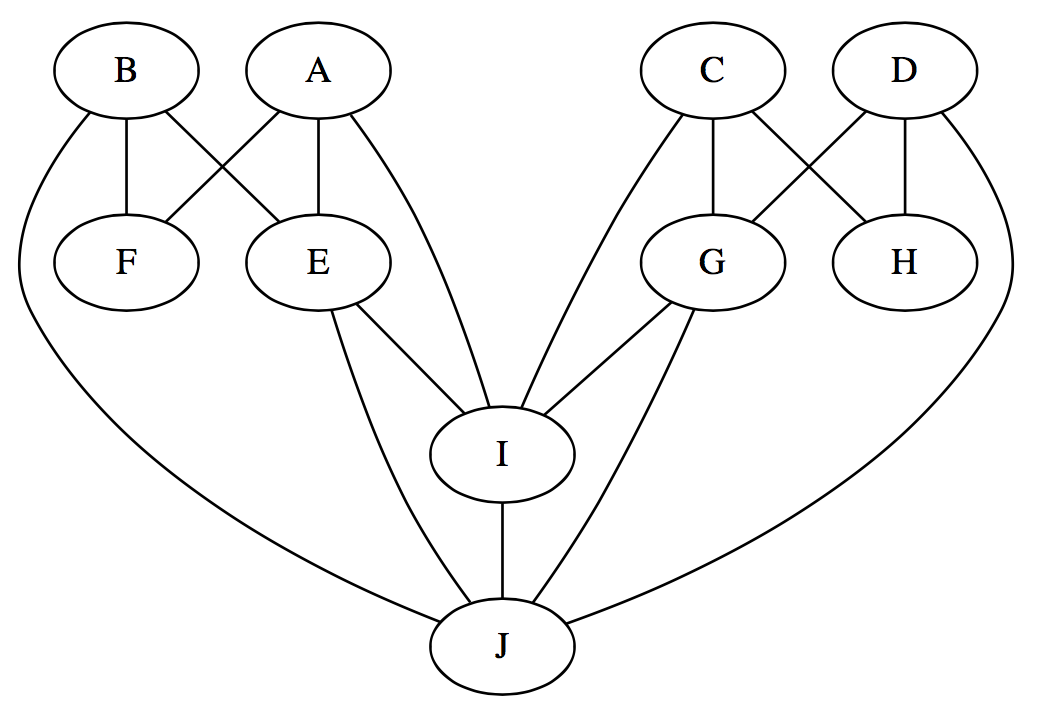
\includegraphics[scale=0.40]{demongraph1}
\end{figure}

\begin{figure}[h]
\caption{Demon2 Graph, V=10 E=17}
\centering
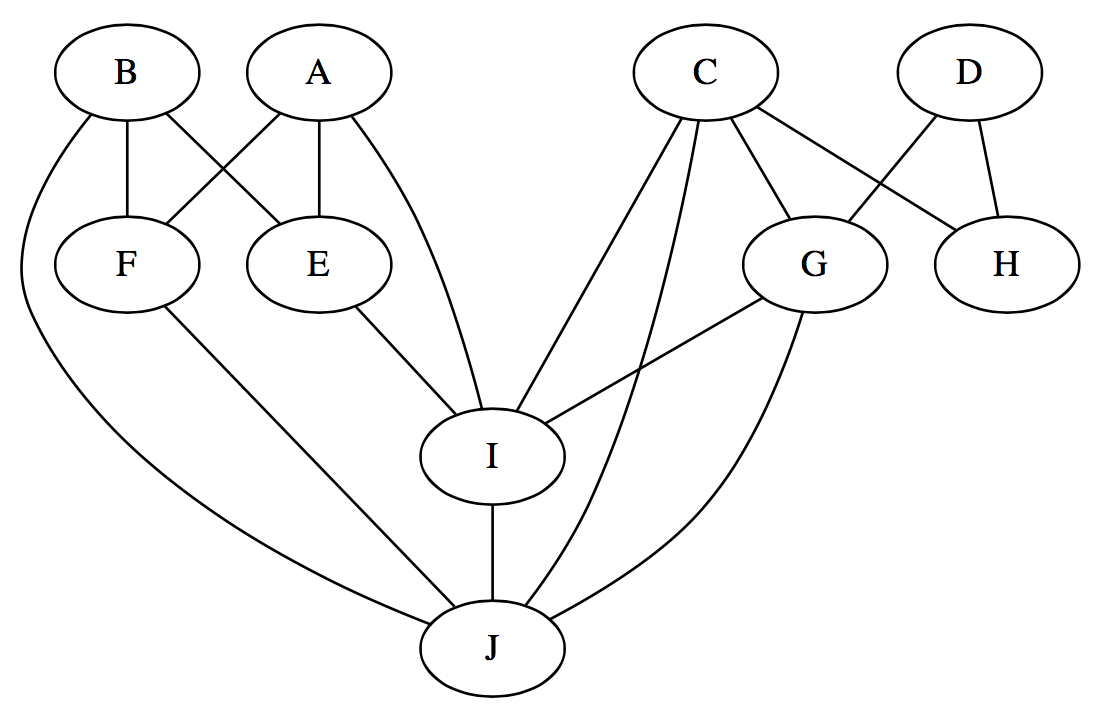
\includegraphics[scale=0.40]{demongraph2}
\end{figure}

Note that actually, more graphs were found that were CoPaths at V=10 and E=17, but they are omitted because I haven't yet deduced any relevant information from them that is worth describing.

Though this section of my semester report is short, it is a notable result, but one that was only discovered recently.  I would expect that this negative result will be the basis for the contributions that my thesis hopes to make on this problem.

\section{The Power Function}

After knowing that Co-Paths, Non-isomorphic graph pairs exist, my focus has shifted from questions of absolute power of differentiability to one of relative differentiating power.  Central to my most recent endeavors in C has been the question: If we take the subset of all non-isomorphic graphs with V vertices and E edges, what is the minimum degree of exponentiation of \(A\) (P), such that all of the paths objects generated by this set of graphs are unique?

This question obviously doesn't have an answer (or at least not a readily computable one) for certain values such as V=10 and E=17, but for smaller values it is not only established that such a threshold must exist, we already have the computational machinery to explore it.

To answer this question, I simply recorded the height of the trie created by the cardinality analysis presented in the coding section.  This height H doesn't describe P directly, but if we take the ceiling of H/V, we get P. We will call the examination of the raw values for H the "granular" approach, and the examination of P as computed by H/V as the "rounded" approach. An interesting comparison can be shown below for graphs of eight vertices. For the purposes of simplicity, the discrete values for P are shown expanded by a factor of V, so that they can be directly compared with H. Note the symmetry, but the noticeable decline in computational power required for graphs with similar number of edges to their complements...

\begin{figure}[h]
\caption{Example Power Paths Function for \(V=8\)}
\centering
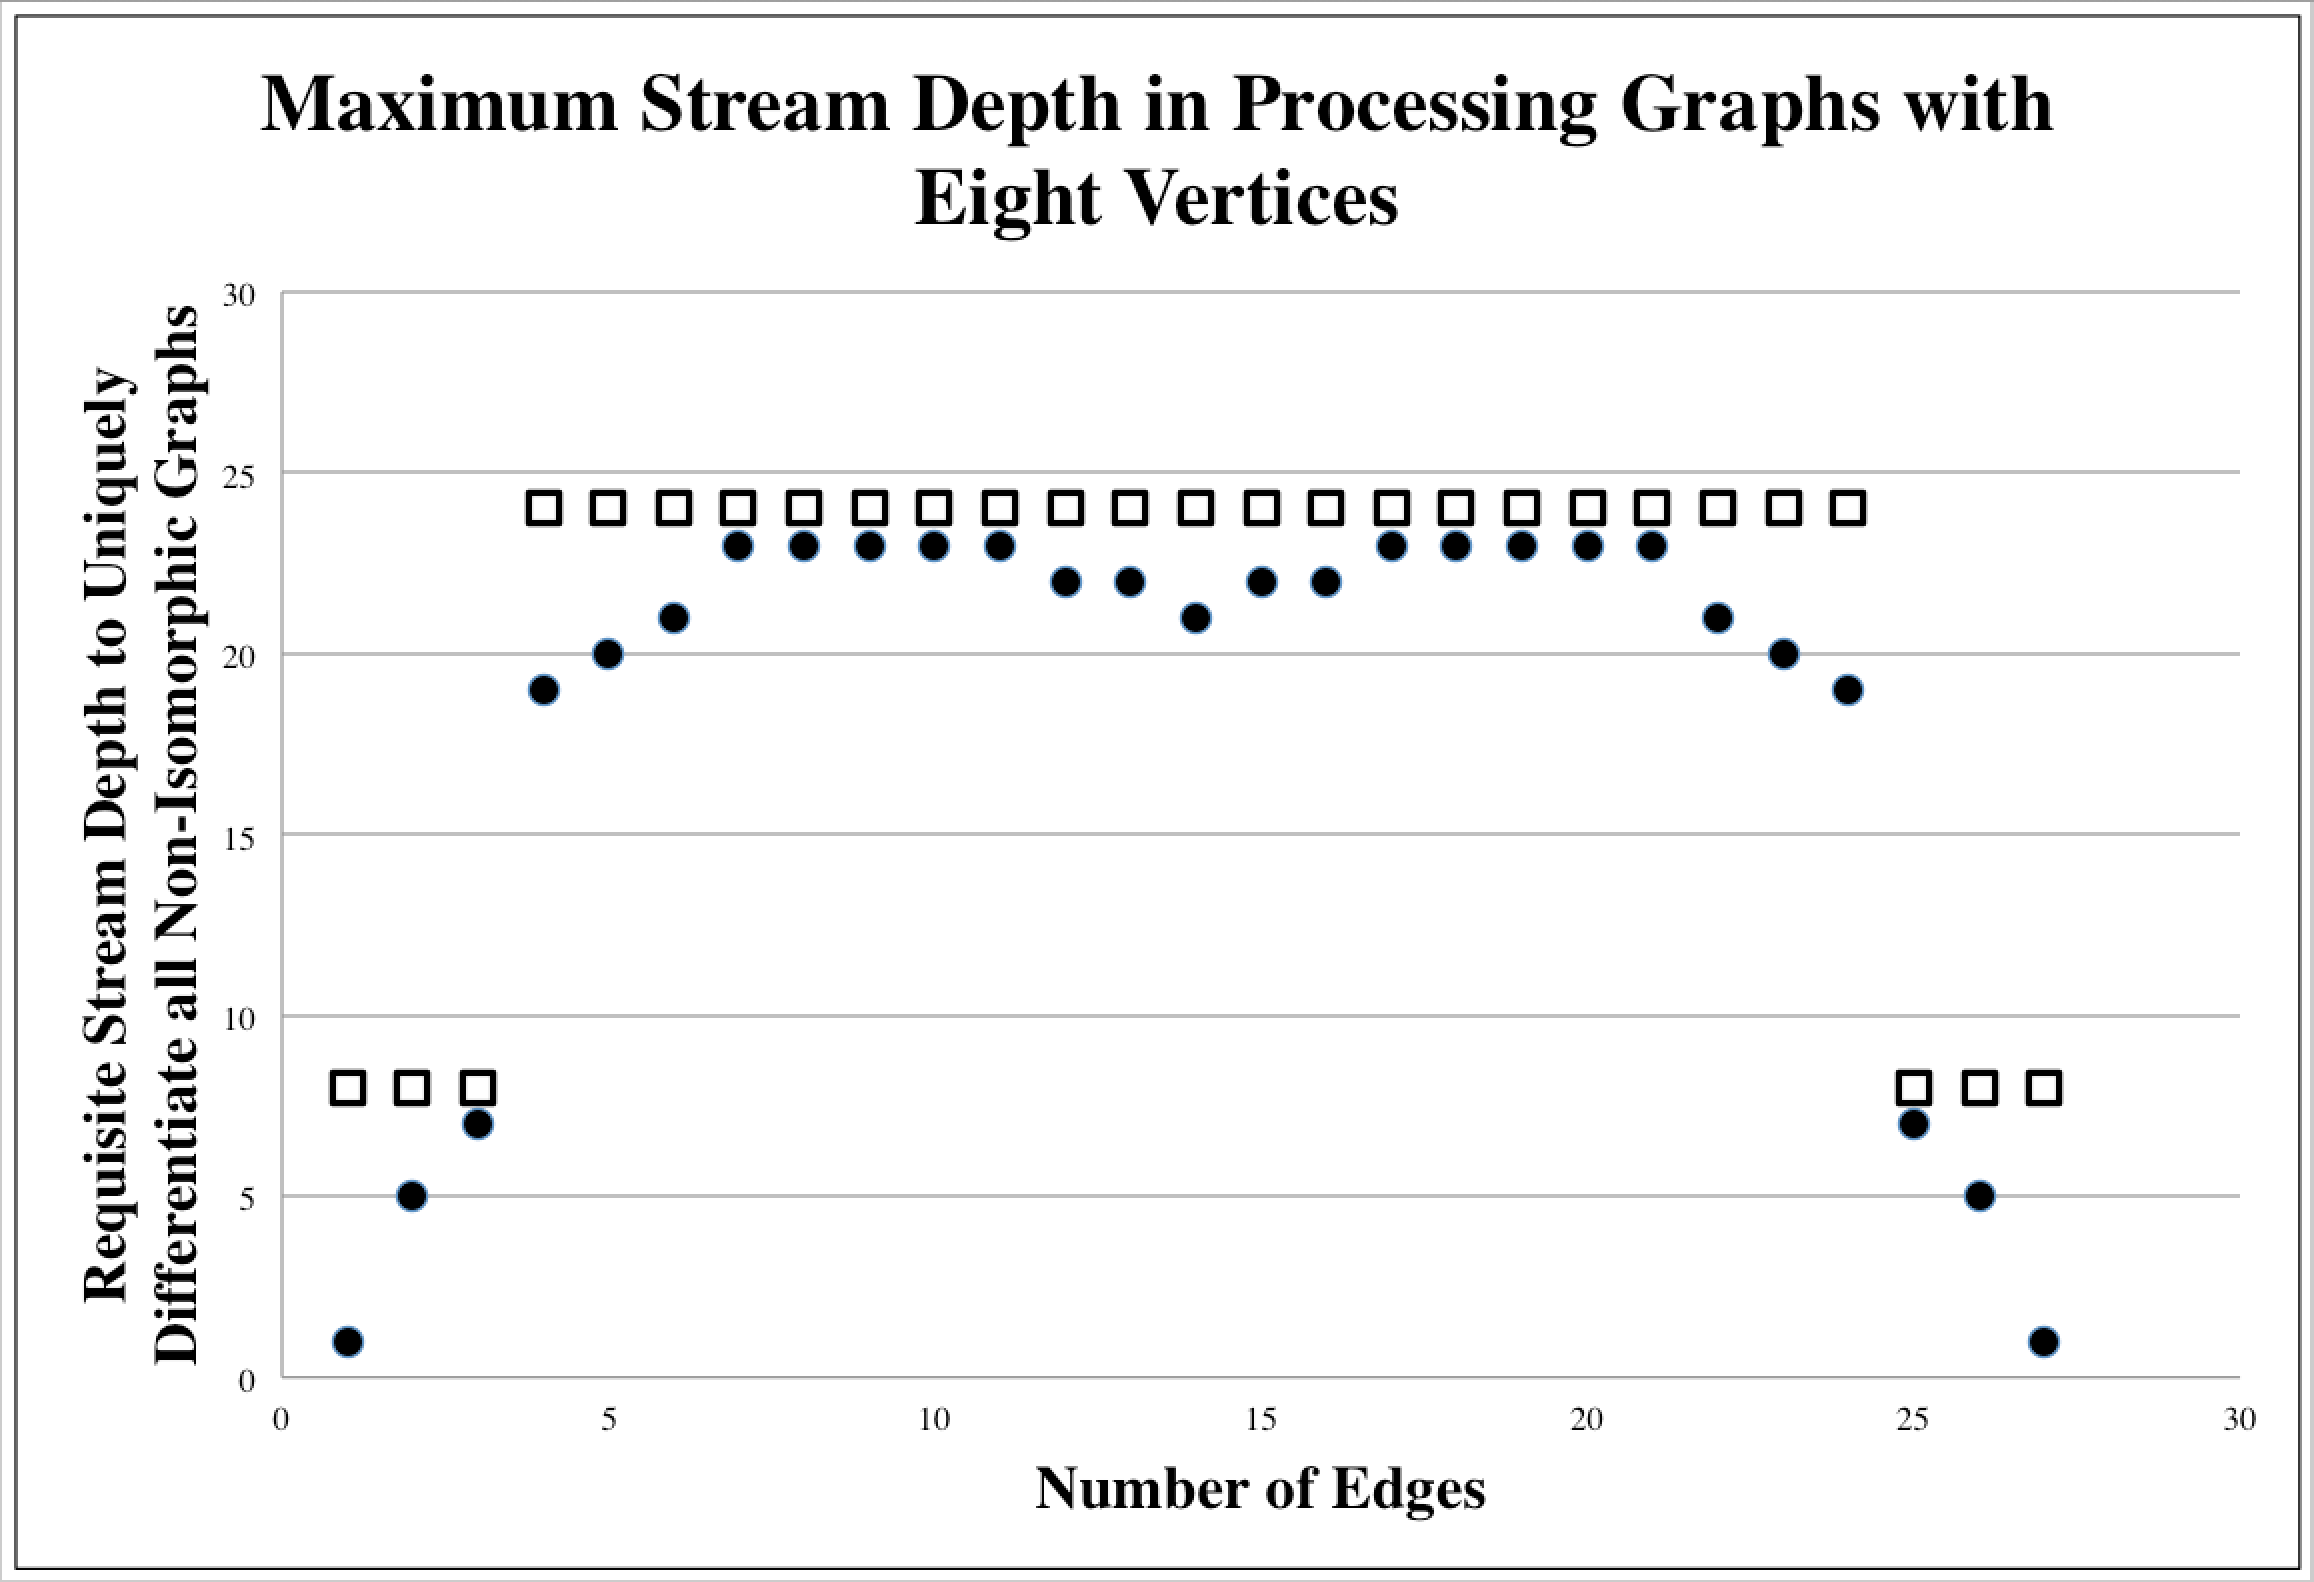
\includegraphics[scale=0.31]{powerfnexample}
\end{figure}

More interesting (but not yet corroborated by two different modes of calculation) is that this pattern doesn't seem to normalize out, but seems to become more dramatic and less predictable as V increases.  Preliminary examination of the power curve for V=9 shows discrete values which actually decrease as the continuous values of H decrease.  This shows that it is not only a process of how we are doing our computation, but \emph{must} be a fundamental property of the computation itself. I have omitted these results because I have some fundamental suspicions about them: the data as I have it recorded is not perfectly symmetric, which one would anticipate would be the case for a problem that inherently is symmetric (i.e. P(V, E) should be the same as P(V, (V*(V-1))/2 - E)). This should be an immediate flag of suspicion, and I look forward to debunking or corroborating these results in the coming days/weeks. 

However, the idea that the discrete values might change alongside the more granular values of H should raise an immediate flag of interest in the mind of anyone who as considered what we would anticipate the power of an algorithm to be relative to its problem definition. We would anticipate that the larger the search size, the lower the absolute power of any given algorithm to determine uniqueness within that space.  Preliminary results from the power paths function computation shows that the opposite may be true. I am very excited to pursue this question further, but will require more time, sleep, and computational power to appropriately address this question, and further pursue this unexpected pattern.

\section{Future Lines of Inquiry}

A thesis is apparently like a Hydra, every time that we answer one question, fifteen more appear.  This independent work has given me a fantastic opportunity to pursue interesting questions that I have discovered as I explore, and given me a taste for academic research and inquiry. Below are some of the questions that are still unanswered moving into next semester, alongside plans for their address and hopeful resolution and analysis. Though I understand that I will not be able to tackle every question that I have, I think that I am well on my way to crafting a thesis which explores this graph invariant robustly, and attempts to marry some graph theory with some thoughtful programming through the exploration of an interesting problem, that hopefully can be shown to be of some kind of practical significance.

\begin{enumerate}
\item Create a program (probably in java) which attempts to verify that paths functions continue to be equal for what we have begun to label as co-paths graphs. We would not want to make the deductive fallacy of assuming that simply because the paths objects line up until the long-integer limit, that that would imply that they line up to infinity. We can verify this claim (at least to a significantly higher degree of accuracy) by utilizing Java's BigInteger class, and hoping to evaluate proposed Co-Paths graphs for absurdly high values of P.
\item Create code which not only attempts to discover the maximum power at which two graphs diverge, but also creates and stores classes of graphs which share the same Paths object as output of this flawed graph invariant.  Code for this purpose will have to be highly fault tolerant, and have to be based on educated assumptions about the reasonable powers that we can assume imply that the number of paths will continue to be the same beyond a large number.
\item Analyze all of the classes of 10-17 graphs, as they are easy to spot the non-isomorphic differences within. What if any features can we compute which differentiate them? Which graph invariants do they agree on? What information can this tell us about the set of graphs for which Paths is uniquely determinate? Moreover, are there broad categorizations of these graphs that might allow Paths to be calculated on the complement set of graphs with a regularity that would befit a correct algorithm for GI, even if it is over a subclass of graphs?
\item Corroborate the results that led to the abnormalities described the Power Paths function through a separate line of brute force inquiry, ideally through something like MATLAB, with high level of accuracy and a reasonable idea of correctness, without trying to duplicate the work that I have obsessed over in C.
\item Explore the Power Paths curve, and try to come up with a unifying way of describing this discrete function.  If we use the granular version of it, how does that change based on our sorting mechanism?  If we use the broad version of it, can we fit some sort of differentiable function to it with a ceiling or round function being used to establish its discrete properties? How can we go about trying to fit three dimensional discrete data when we know (or suspect) that some of our resulting values are infinite?
\item Explore the power paths curve in granular detail: what percentage of all graphs fit into classes that are co-paths?  What is the average depth of a leaf within this Trie, and what is the average differentiating power of two graphs?  Each of these metrics sounds really interesting, and is certainly computable. There was a large surprise in the overall shape of the Power Paths function; what other secrets and patterns lie in this function which characterizes the descriptive power of the paths function, and the inherent complexity of the Graph Isomorphism problem?
\item Extend the logic of the existing C program to one which uses virtual memory and stream processing from the GENG graph generator.  Currently the limitation that our program runs in to is not one of speed, but one of memory allocation and access.  This should not be surprising when we are allocating at least one node, two matrices, and three arrays for each of the graphs, and the number of graphs is in the trillions.  We can spare some speed on the computation side if we can use it to shift toward a disk intensive set of operations.  Deciding how that will take place, and the role of multi-processing in that endeavor is a large task, but may allow us to extend existing methodologies to explore the areas of \(V>11\).
\item Explore theoretical justification for low-paths determinism: why is it that we see that most graphs are either 1) fully determined by paths at a relatively low value of P (usually linearly defined with respect to V), while others appear to exponentiate identically to infinity? Why does this divergence exist? Wouldn't we anticipate that in a system like this we would see some sort of normal distribution?  What can we say about this threshold if it exists?  Are there theoretical reasons (intuitive or in algebraic graph theory) that can explain this phenomena? My intuition says that this has something to do with the algebraic polynomials discussed in previous reports, and the fact that their degree is fixed as a linear function of V and E, while our paths function is allowed to wander up toward infinity...
\item When I reach a point that my data is able to draw a picture without holes, email the Cornell professor who originally proposed this invariant, and discuss it with him.
\item Closely examine the relation that sets of Co-Paths graphs appear to have (properties of the sets, not of the graphs themselves, which will be a separate analysis). We have to realize that these sets are bound to be linked through some sorts of inverse, concatenation and union operations, and that they may be linked in ways that are more profound that we can yet imagine.
\item Set upper bound worst case approximations for the number of bits that are necessary to calculate, store and compare the Paths Object for a given value of V, E and P. Invert this function to create a calculator for the maximum size we could create for a given chunk of allocated memory.
\item A question that I asked several months ago has suddenly (with the discovery of co-paths graphs) become significantly more important: what are the information density bounds on the Paths Function? Clearly this is a topic that will broadly be the focus of the next semester of research and development, but we can refocus work on this topic while maintaining lines of inquiry that tap into broader questions about the nature of \(Paths\), and its place (if any) within the Graph Isomorphism Problem.
\end{enumerate}

\section{Conclusion}
This has been a wild semester.  I have discovered patterns I have not expected, found the existence of counterexamples to my original hypothesis, and begun exploration of the patterns inherent in these counterexamples.  Moreover, I have learned a great deal in programming (including any programming in C and OpenCL), and a great deal in algebraic graph theory.  I think that I have a good amount of work ahead of me in the coming semester, but I am more excited than ever to try and answer some of the questions that have yet eluded me, or just recently come to my attention. I would like to sincerely thank my Advisor Prf. Jim Storrer for being a delight to talk to about these problems, guiding my questions and ideas, giving me access to the computational resources that I need to pursue those ideas, and indulging my whims about researching for the fun of it all.

\end{document}